%% This is an example first chapter.  You should put chapter/appendix that you
%% write into a separate file, and add a line \include{yourfilename} to
%% main.tex, where `yourfilename.tex' is the name of the chapter/appendix file.
%% You can process specific files by typing their names in at the 
%% \files=
%% prompt when you run the file main.tex through LaTeX.

\singlespacing{

\chapter{Simulation of Functional Digital Materials}\label{chap:functionSim}

Simulation of function-level parts is carried out through a mass/spring/damper model.  In this model, neighboring face-connected cells apply forces and torques on one another through local interactions.  Translational and rotational positions and velocities are calculated from these forces using discrete-time integration techniques.  Internal degrees of freedom of \textit{functions} are parameterized by 15 stiffness and damping coefficients, $k$ and $d$.  Actuation is achieved by modulating the nominal distance of adjacent cells along a particular degree of freedom.\\





This thesis is concerned only with the linear elastic deformation of solids, in other words, things that obey Hooke's law:

\[F = kx\]

where F is a force, x is a displacement, and k is a material stiffness.  In the form above, $k$ depends on the geometry of the material, it is a measure of \textit{geometric stiffness}.\\

FEA is essentially the process of applying Hookes law over and over to small regions of a volume and summing up their net solution.


\section{Existing Models of Solids}

\href{https://en.wikipedia.org/wiki/Solid_mechanics}{Solid mechanics} is the study of the motion and deformation of solid bodies under external forces, changes in temperature, and other stresses.  Solid mechanics differentiates itself from other branches of continuum mechanics because solids are assumed to have a preferred rest shape.  This thesis is concerned with a subset of solid mechanics called elasticity, where materials return to their initial rest shape after all external forces are removed. \\

The behavior of elastic solids is usually described by stress and strain.  Stress describes the internal forces acting on neighboring regions of a material, measured as force per area in pascals (PA) or N/m\textsuperscript{2}.  Strain describes the deformations of these regions in response to stress, measured as a unit-less ratio of a length of deformation per unit of unstressed length.\\

This thesis explores both isotropic and anisotropic materials.  A material is isotropic if it responds the same to an external force no matter its orientation; materials comprised of oriented fibers or other directional structures typical display anisotropic behaviors.  The response of solids to strains are typically expressed in terms of their elastic modulus $E$ and shear modulus $G$, however, for anisotropic materials, such as those used in our assembly system, this parameterization does not give enough information.\\


%\subsubsection{Simulation Techniques for Solids}

This thesis is concerned with the numerical solution of the position, orientation, and deformation of an elastic solid made from many elements of identical geometry and various material types.  Based on the distribution of elements and material types throughout the solid, it is possible to describe its dynamic behavior with a \href{https://en.wikipedia.org/wiki/Partial_differential_equation}{partial differential equation} (PDE).  Evaluating this PDE subject to the initial state and boundary conditions (applied forces, fixed regions, etc) gives the state of the solid over time.  There are a few different techniques for doing this; depending on the specific requirements of a simulation, it may be more advantageous to use one over another.\\

The first technique is called the \href{https://en.wikipedia.org/wiki/Finite_difference_method}{Finite Difference Method} (FDM).  \\


A more complete discussion of FDM, FEM, and FVM is given in Peiro et al.\cite{Peiro2005}.\\

FEA vs Mass-Spring vs CA\\
few works well for linear - non linear for large deformations may require remeshing\\
mass spring methods - widely used in computer graphics, better for large deformations and non linear, less accurate\\
differential elements\\

Mass/spring/damper
FEA

%Unlike traditional mass/spring/damper models of solids from computer graphics literature (cite stuff here), the model developed in this thesis draws on an abstraction of the functionality embedded in the different "function types".

\begin{figure}
  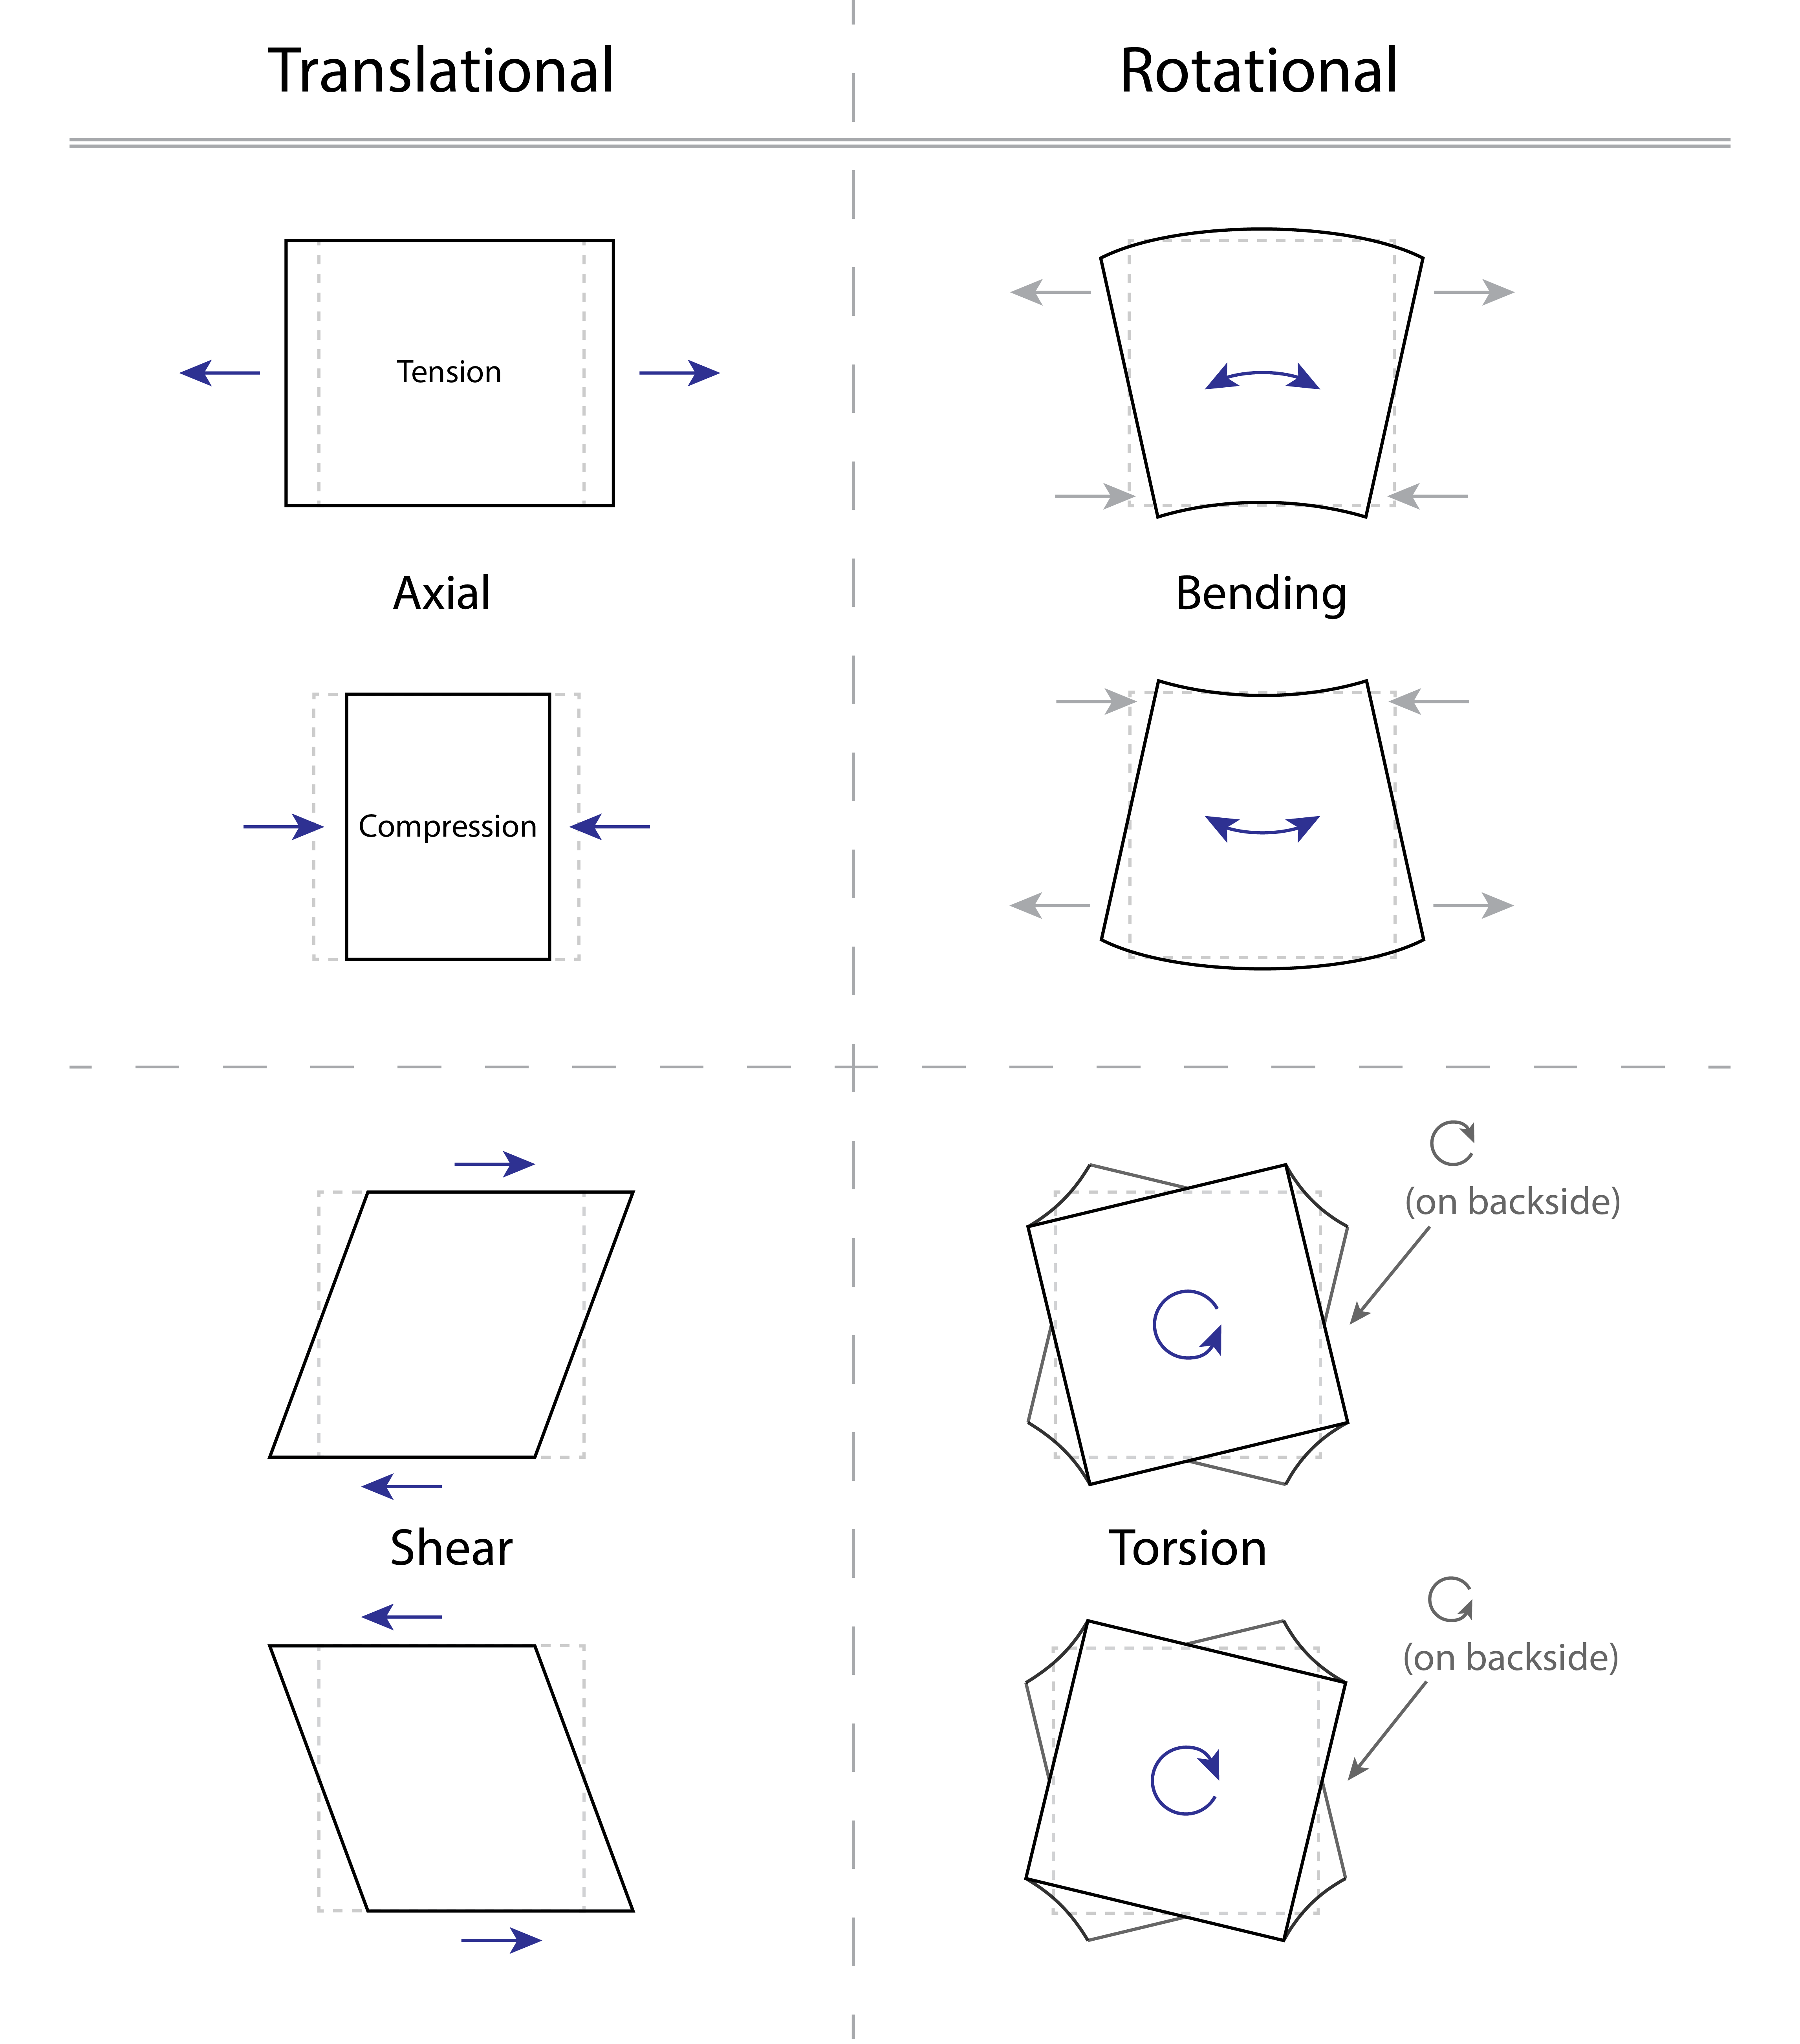
\includegraphics[width=\linewidth]{SolidMechanicsDOF.png}
  \caption{Deformations of a solid element under four types of applied forces.  In modeling assemblies of \textit{functions}, these characteristic deformations are referred to as "internal degrees of freedom".  Within an assembly of cells, longitudinal (compression and tension) and shear forces cause translational displacement and bending and torsional forces cause rotational displacement.}
  \label{fig:SolidMechanicsDOF}
\end{figure}

In solid mechanics, we can consider the global deformations of a solid as the summation of deformations of many smaller, discrete volumes, or \textit{finite elements}.  Forces acting on these finite elements fall into four categories: longitudinal (tension and compression), bending, shear, and torsion.  Each type of applied force causes a characteristic deformation of the finite element, illustrated in Figure \ref{fig:SolidMechanicsDOF}.  Applying multiple types of forces on a finite element will cause it to exhibit a combination of deformations.\\

In this model, simulation of an assembly happens at the granularity of identically-sized \textit{function}-level parts, which we'll call "cells".  When describing mechanical behavior of a particular cell type, we refer to its deformations as "internal degrees of freedom" (DOF).  For example, a 1-DOF bending cell will have large deformations in bending along one axis, but relatively small deformations in response to other types of applied forces.\\


}
